\documentclass[journal]{new-aiaa}
%\documentclass[conf]{new-aiaa} for conference papers
\usepackage[utf8]{inputenc}
\usepackage{graphicx}
\usepackage{amsmath}
\usepackage[version=4]{mhchem}
\usepackage{siunitx}
\usepackage{longtable,tabularx}
\usepackage[section]{placeins}


%\usepackage{cite}


\setlength\LTleft{0pt} 

\title{Perceptron Q-learning applied to Super Smash Bros Melee}

\author{Liam Brown \footnote{Graduate Student, Aeronautics and Astronautics.} and Jeremy Crowley\footnote{Graduate Student, Aeronautics and Astronautics.}}
\affil{Stanford University, Stanford, CA, 94305}

\begin{document}

\maketitle

\begin{abstract}
Reinforcement learning (RL) is able to produce effective policies in environments with small discrete state and action spaces but has significant limitations when the state-action space is continuous. Discretization techniques can solve the issue of continuous state-action spaces, however this often results in intractable state spaces or a poor approximation of the continuum.In this paper, we discuss a reinforcement learning strategy for t Super Smash Bros Melee, a video game with a continuous state and action space by applying global approximation in the Q-learning algorithm. We train the algorithm on progressively harder opponents and show improvement in the agents metrics over time.

\end{abstract}


%
% Introduction
%

\section{Introduction}
\lettrine{S}{uper} Smash Bros Melee presents a state space with complex dynamics that is difficult to model without knowledge of the source code used to build the game. 


%
% Related Work
%
\section{Related Work}

Q-learning has been studied for the past few decades due to its ability to learn complex tasks without little knowledge of the underlying system. While reinforcement learning can prove to develop desirable policies, knowledge of the environment the agent is acting is is crucial. Often times, the state space and action spaces are continuous, and difficult to represent like in~\cite{gaskett} where Gasket et al implemented a novel interpolator to approximate the Q-function with state generalization and action generalization. In addition to the difficulties continuous state and action spaces present, environments can be adversarial. Applying reinforcement learning in an adversarial environment can prove to be difficult because the environment is working against the agent. In~\cite{uther}, a generalized reinforcement learning algorithm is applied to a agent in an adversarial environment. Both~\cite{gaskett} and~\cite{uther} show that applying generalization to reinforcement learning is viable solution to dealing with the complexity of discretizing state and action spaces. 

In more recent advancement in generalization for reinforcement learning, Emigh et al applied a local approximation reinforcement learning algorithm in~\cite{emigh} to a video game called Frogger. Nearest neighbor  is a local approximation method to generalize the state space based on states that close in proximity to each other. This proves to be a good strategy when there is limited data and the optimal policy can still prove effective is applied to states close to previously visited states.

Another difficulty in reinforcement learning is assigning credit to the action the led to the reward. Depending on the dynamics of the environment that reinforcement learning is being applied to, the reward from executing an action can be delayed. Take for example winning the lottery, there is a large delay between when we but the lottery ticket and when we get the reward. If we are drinking coffee right before we find out we win the lottery, the reward of winning the lottery should still be assigned to buying the ticket and not to drinking coffee. Sutton et al developed a method in~\cite{sutton} to properly assign credit to the action or sequence of actions that lead to a reward. This problem can become increasingly difficult to address as the dimensionality of the problem increases.





hurt dur t \cite{sutton}




%
% Applications to Super Smash Bros Melee
%
\section{Applications to Super Smash Bros Melee}
- state evolver / intractable state space / discretized controller

\subsection{Discretized actions}
The controller for the Nintendo game cube can be thought of as a continuous action space for Super Smash Brothers Melee. There are two analog control sticks which can be placed at any value from -1 to 1 in both the x and y direction, two analog shoulder buttons which are functionally identical and range from 0 to 1, as well as four digital face buttons. 

To reduce the number of potential actions, repetitive combinations of buttons were discarded and the analog inputs were discretized. We represented five buttons ($A$,$B$,$X$,$L$, and $Z$) as binary variables, where a value of one maps to pressed and zero maps to not pressed, and the analog stick as a variable with three possible values for both the x direction, $N^{x}$, and the y direction, $N^{y}$. We also include a "short hop" button press, $X_{s}$, where X is pressed for a shorter amount of time, and a "none" button press, $\varnothing$, where none of the buttons are pressed. 

To create an action, we select a single button and a direction for the analog stick. Recall we have seven possible button presses ($A$,$B$,$X$,$X_{s}$,$L$,$Z$, $\varnothing$) and nine possible analog stick values. This results in an action space $\mathbb{A}$ with size 63.


\subsection{Basis Functions}
Since our project is based on perceptron Q-learning we designed a set of basis functions to span the state space SSBM. Our beta vector, $\beta$, contains the following elements.

\begin{itemize}
\item A set of normal distributions along the x and y axes
\item A set of normal distributions for the relative distance between the agent and the opponent
\item A flag for the direction the agent is facing and a flag for the direction the opponent is facing
\item A set of flags for the agent and a set of flags for the opponent to represent unique animations
\item A set of normal distributions for the agent and opponents damages
\item A set of flags for the number of jumps left
\end{itemize}

We employed an interesting strategy to have our agent behave differently when it is off the map (i.e. about to die and needs to perform a recovery move to get back on stage) versus when it is in the middle of the map. We split the map up into left, middle, and right. Instead of using the beta vector as constructed in the list above, we make a zero-padded version of the beta vector depending on where the agent is in the map. For example, if the agent is on the left side of the map we create a padded beta vector, $\beta_{p} = [\beta,~0_{|\beta|},~0_{|\beta|}]$, where $0_{|\beta|}$ denotes a vector of $|\beta|$ zeros. Similarly, when the agent is in the middle of the map our beta vector becomes $\beta_{p} = [0_{|\beta|},~\beta,~0_{|\beta|}]$ and when the agent is on the right side of the map our beta vector becomes $\beta_{p} = [0_{|\beta|},~0_{|\beta|},~\beta]$. This effectively results in differently trained perception weights, $\Theta$, for the different map partitions.

\subsection{Reward Functions}

In order to apply perceptron Q-learning to to SSBM, we defined a reward function and a set of basis functions. As described in the introduction, the goal of the game is to ultimately knock your opponent off the stage, which becomes easier as their damage increases since the damage causes them to fly further. This indicates a careful balance between accumulating damage to facilitate a knock out move, and overly focusing on accumulating damage with no regard for the ultimate goal of getting a knock out. To tackle this, we defined the reward function between states to include a decay for damage dealt when the opponent is already at higher percentages, as well as a penalty for taking damage. In order to prevent suicidal behavior of the agent, a reward was also given when the agent managed to move from being off of the side of the stage in state s, to on the stage in state $s'$

Denoting the opponents damage as $d_o$, the agents damage as $d_a$, and the on stage parameter of the agent as a true / false flag $ON$, the reward function became:

$$R = (d'_o-d_o)exp(-.01*d_o) - (d'_a-d_a)exp(-.01*d_a) + \delta_{0,ON}\delta_{1,ON'}$$

In addition to this reward given out at each state transition step, a novel method for assigning rewards to significant important states was formulated. To assign rewards to killing the opponent, the last action the agent took that resulted in an increase in damage to the opponent is recorded. When the opponent dies, a large reward is assigned to this "last damaging action". This is due to the long lag between hitting the opponent and them dying, and the necessity of avoiding assigning large rewards to actions that had nothing to do with the opponnent dying. 

Additionally, a finite length action history is tracked for the purposes of assigning negative rewards to deaths. When the agent dies, all actions in the action history are penalized, as the agent could have taken an action in this time frame that may have prevented its death but ultimately chose not to. An example of this is the agent being slightly off the edge of the stage and not choosing to jump back on. The action selected instead of jumping back on is then penalized.





%
%Novel approaches to state evolution
%
\section{Unique Approaches}

To apply perceptron Q-learning to Super Smash Brothers Melee, we apply unique techniques to deal with discontinuities in optimal behavior, state-evolution, and large delays between an action and its result.

\subsection{Discontinuity in Optimal Behavior}
In Super Smash Brothers Melee, the optimal action largely depends on the current state. An issue arises in global-approximation techniques when states that produce similar basis function outputs should have dissimilar optimal actions. An example of this is the case of an agent standing on the edge of the stage, in which its goal is to deal damage to the opponent, and an agent being slightly off of the stage (about to fall to its death unless some preventative action is taken), in which it should make an effort to navigate back to the stage and avoid dying. 

To prevent generalization from nearby but dissimilar states, we discretize the environment into an additional three "super-states": off the stage to the left, on the stage, and off the stage to the right. These super-states represent different situations in which the optimal behavior of the agent should be unique from a nearby position that is in a different super-state. As discussed in the applications section, the padded beta vector results in differently trained perceptron weights in different super-states for each map partition. This improves the agents ability to survive after being knocked off of the stage because the agent learns to jump back towards the stage in an effort to survive (and avoid penalties for dying). 

\subsection{State Evolution}
Another issue we address was the impact of ”action-lockout”, in which an action taken may have no impact on the agents transition to the next state. An example of this is when the agent selects an action with a long wind-up animation that cannot be canceled by inputting other actions. To address this, actions that are taken during an "action-lockout" are ignored during the training process of the basis function weights. 

While performing batch learning, this is taken into account. In the weight update process, $\theta_a\beta(s)$ of the last action take is used for each update, while the state $s'$ is taken as usual. The rewards are computed at each state step and assigned back to the last action taken. The result is that the original state action pair is rewarded for the state evolution that occurs, rather than rewarding the action at intermediate states of the evolution. 

\begin{figure}[!htb]
	\centering
	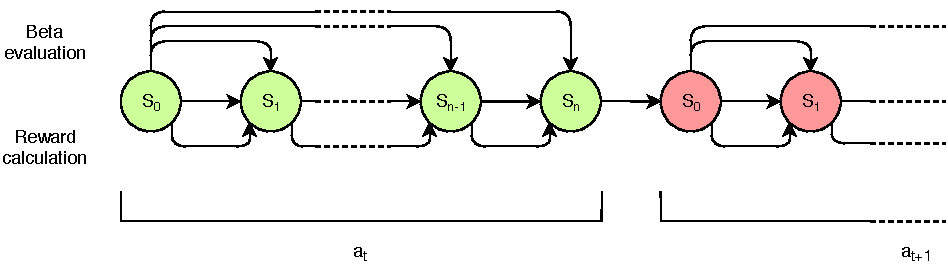
\includegraphics[width=120mm]{stateevolution.pdf}
	\caption{State evolution diagram}
	\label{fig:stateevo}
\end{figure}

Figure~\ref{fig:stateevo} is a representation a state evolution. All the green states indicate a single state evolution with action-lockout occurring at each new state $S_{t}$. The transition to the red states are when an action is taken that affect the transition to the next state, starting a new state evolution. We can see the how the reward is calculated from $S_{t}$ to $S_{t+1}$ while the beta function is evaluated from $S_{0}$ to $S_{t+1}$.

\subsection{Action Impact Delay}

Dealing with rewards for kills and deaths is not straight forward due to a large time delay between an action that results in one of these events and the event occurring. To assign rewards to killing the opponent, the last action the agent take that deals damage is recorded as a "last damaging action". When the opponent dies, a large reward is assigned to this "last damaging action". This is necessary to avoid assigning large rewards to actions that do not cause the opponent to die, and is equivalent to knowing immediately after the action is taken if it will result in the death of the opponent.



%
% Results
%
\section{Results}
The agent was initialized with no prior against a level 1 CPU and was allowed to train overnight, training the weights between each match. For training, we used a learning rate of $\alpha = 0.01$, a discount factor of $\gamma = 0.95$, and a non-fixed soft-max exploration parameter $\lambda$. The agent was trained against progressively harder opponents while using priors from the previous training, until we reached a level 4 CPU.

In Figure~\ref{winpctg}, we see that the uninformed agent with a high exploration bias quickly achieves an approximately 80 percent win-rate against the base level 1 opponent. When this agent is then given a lower exploration bias, that win-rate quickly converges to 100\%. The first real challenge faced is against the level 3 opponent, were the agent undergoes a difficult period, having its win-rate fall to near 50\% before recovering back to 100\% over a period of approximately 100 games. A similar trend is observed when the agent faces off with a level 4 opponent. We can also see similar trends in Figures~\ref{stocks}, and~\ref{damage} where the stock differential and the damage differential slowly improve as the agent trains. 

In addition to the quantitative performance metrics observed in the Figures, the agents behavior also improved qualitatively. Against the level 1 opponent, the agent learned basic behaviors that lead to a win. The agent would simply repeat the same attacking move that the level 1 opponent was unable to deal with. As the agent faced progressively more difficult opponents (level 3 and 4), this behavior would sometimes work but would often result in the agent taking damage. The agent was able to determine states in which this learned "spamming" behavior was optimal and which states it should avoid, and developed new strategies depending on the state.

An interesting trend in the data is the increase in games required for the agent to learn an effective policy against its opponents. Against the level 1 CPU, we see that the winning strategy can be learned in approximately 85 games. Against the level 3, this process takes 85 games, and against the level 4 CPU we were only able to achieve an 85\% winrate after 245 games. 



%Beginning from no prior knowledge, the agent quickly progressed to wining games against its opponent, preserving its own stocks, as well as increasing its relative damage output. This trend carries over into the other sessions as well and can be observed in figures ONE TO THREE. An interesting note is that the performance of the level 1 CPU trained agent against the level 3 CPU initially declines from its initialized behavior before recovering to a 100 percent win-rate. 




%
% Conclusion
%
\section{Conclusion}

Applying perceptron Q-learning for Super Smash Brothers Melee was successful. Given enough time, the agent learned to progressively beat higher level default CPUs, die less, and take less damage. One severely limiting factor of the project was the need to run the agent in real time against a CPU in order to train. This caused iteration on the basis functions, reward functions, hyper parameters as well as progression through CPU difficulty to be slow. On the other hand, the combination of our achieved performance and low iterations on parameters and functions shows the robustness of perceptron Q-learning in this environment. 

We believe that with improvement to the reward functions and careful detail to to hyper parameters, as well as more time, the agent could learn to beat significantly higher level CPUs than demonstrated here. Additionally, while the agent has only ever played as captain falcon against captain falcon, the agent should be able to learn to play any matchup and on any stage. This could be done by storing different basis function weights for each situation.

Our group plans to continue the project by both continuing to play against higher level agents with the existing perceptron Q-learning approach, as well as extending the bots capabilities by implementing DQN. We believe DQN will provide a higher level of performance as it is able to represent non-linear basis functions, while perceptron Q-learning is limited to linear relationships. We are also looking to explore different characters and stages.




%
% Appendix
%
\newpage
\section*{Appendix}

\begin{figure}[!htb]
\centering
	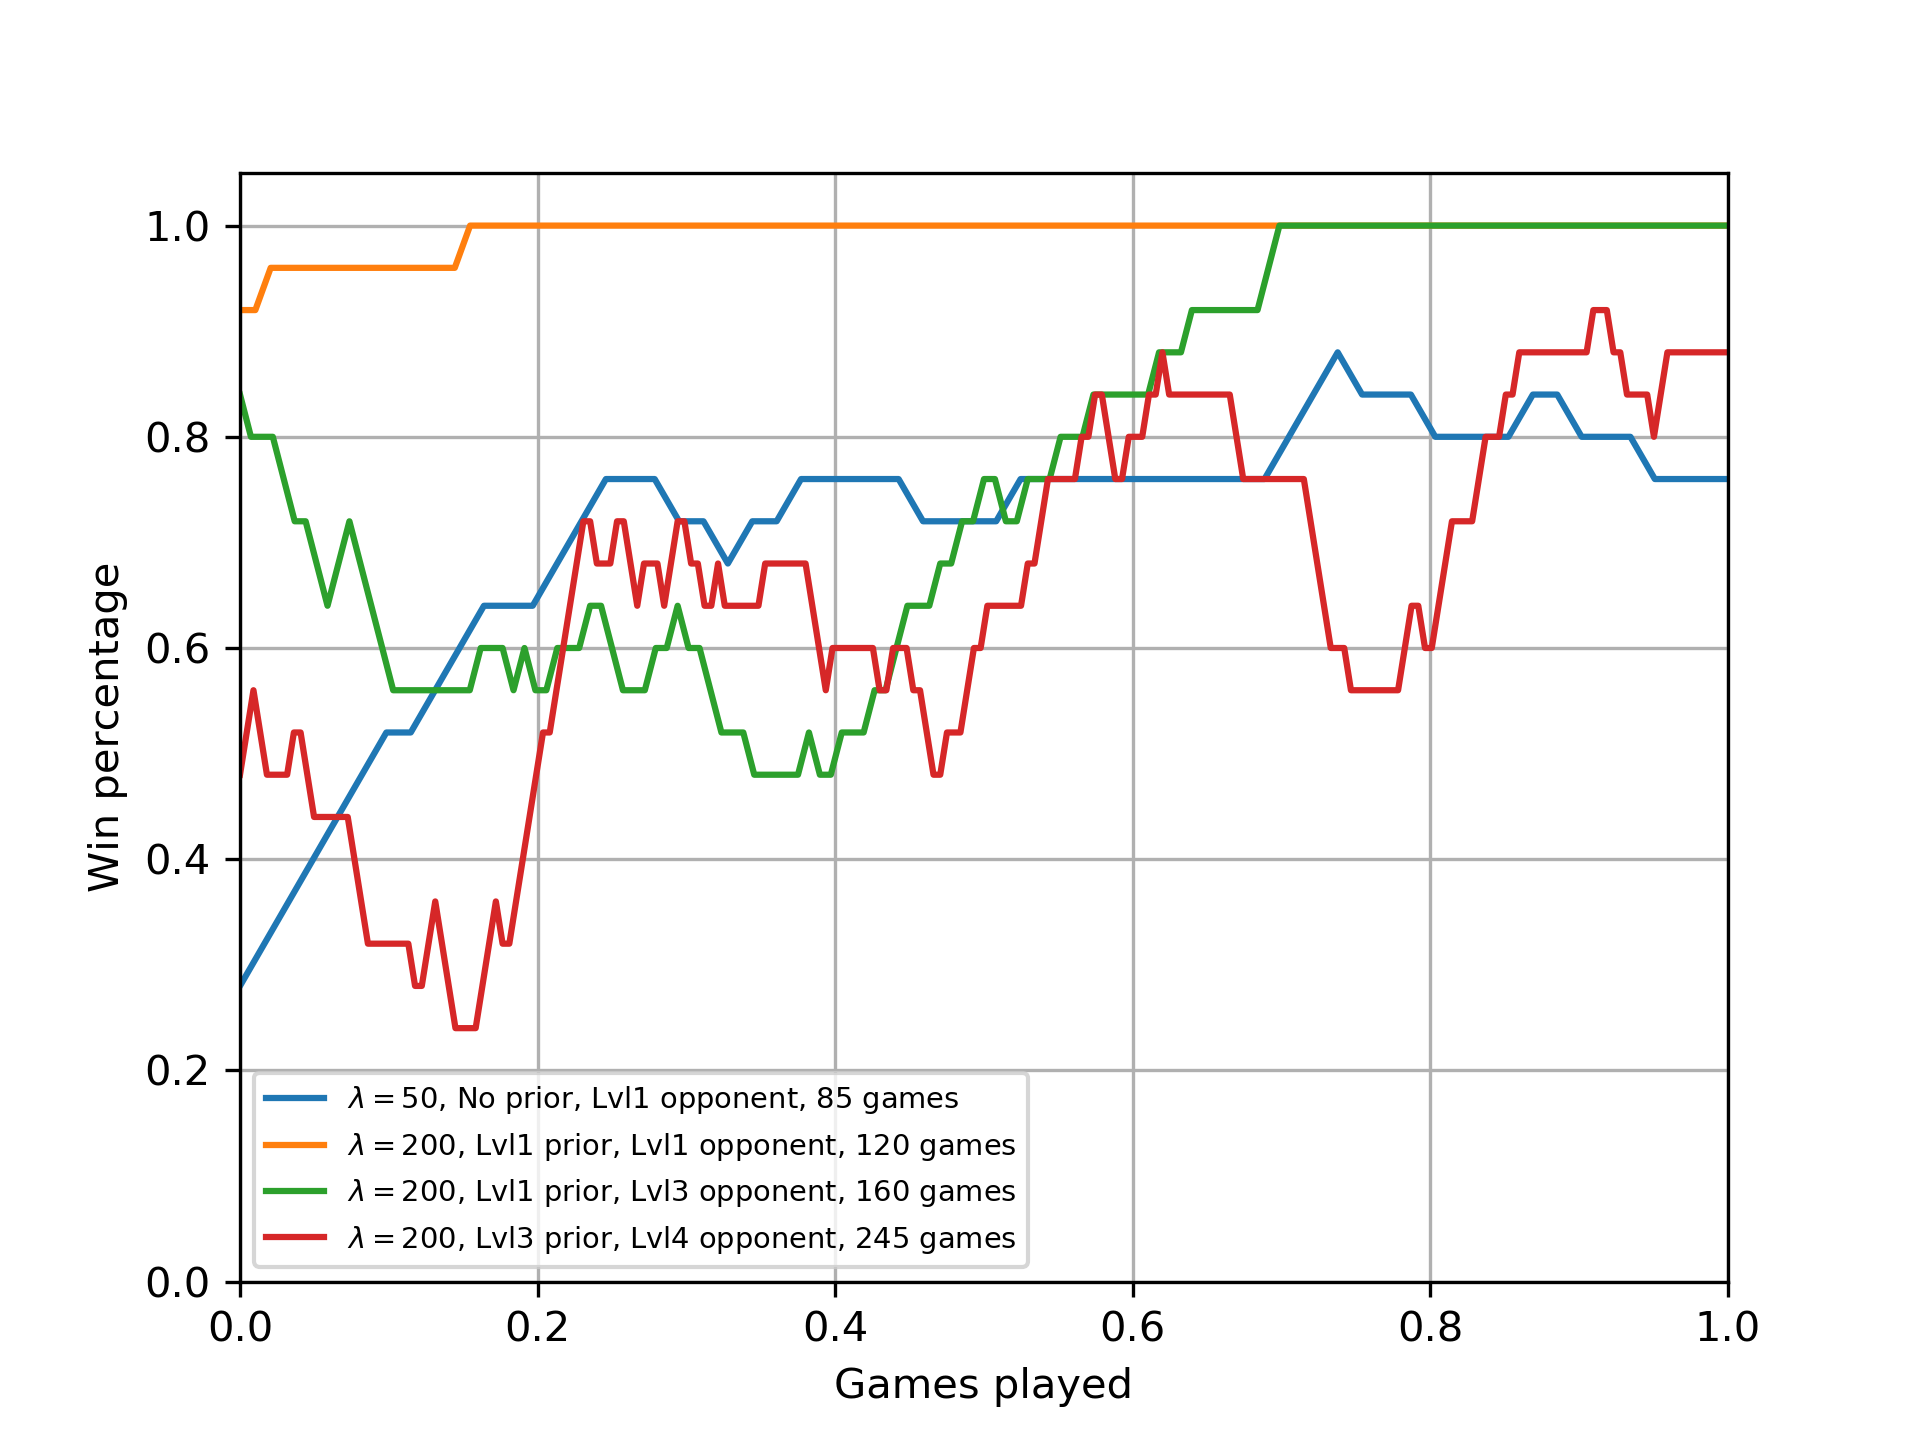
\includegraphics[width=120mm]{winpctg.png}
	\caption{25 game moving average of winning percentage. \label{winpctg}}
\end{figure}

\begin{figure}[!htb]
\centering
	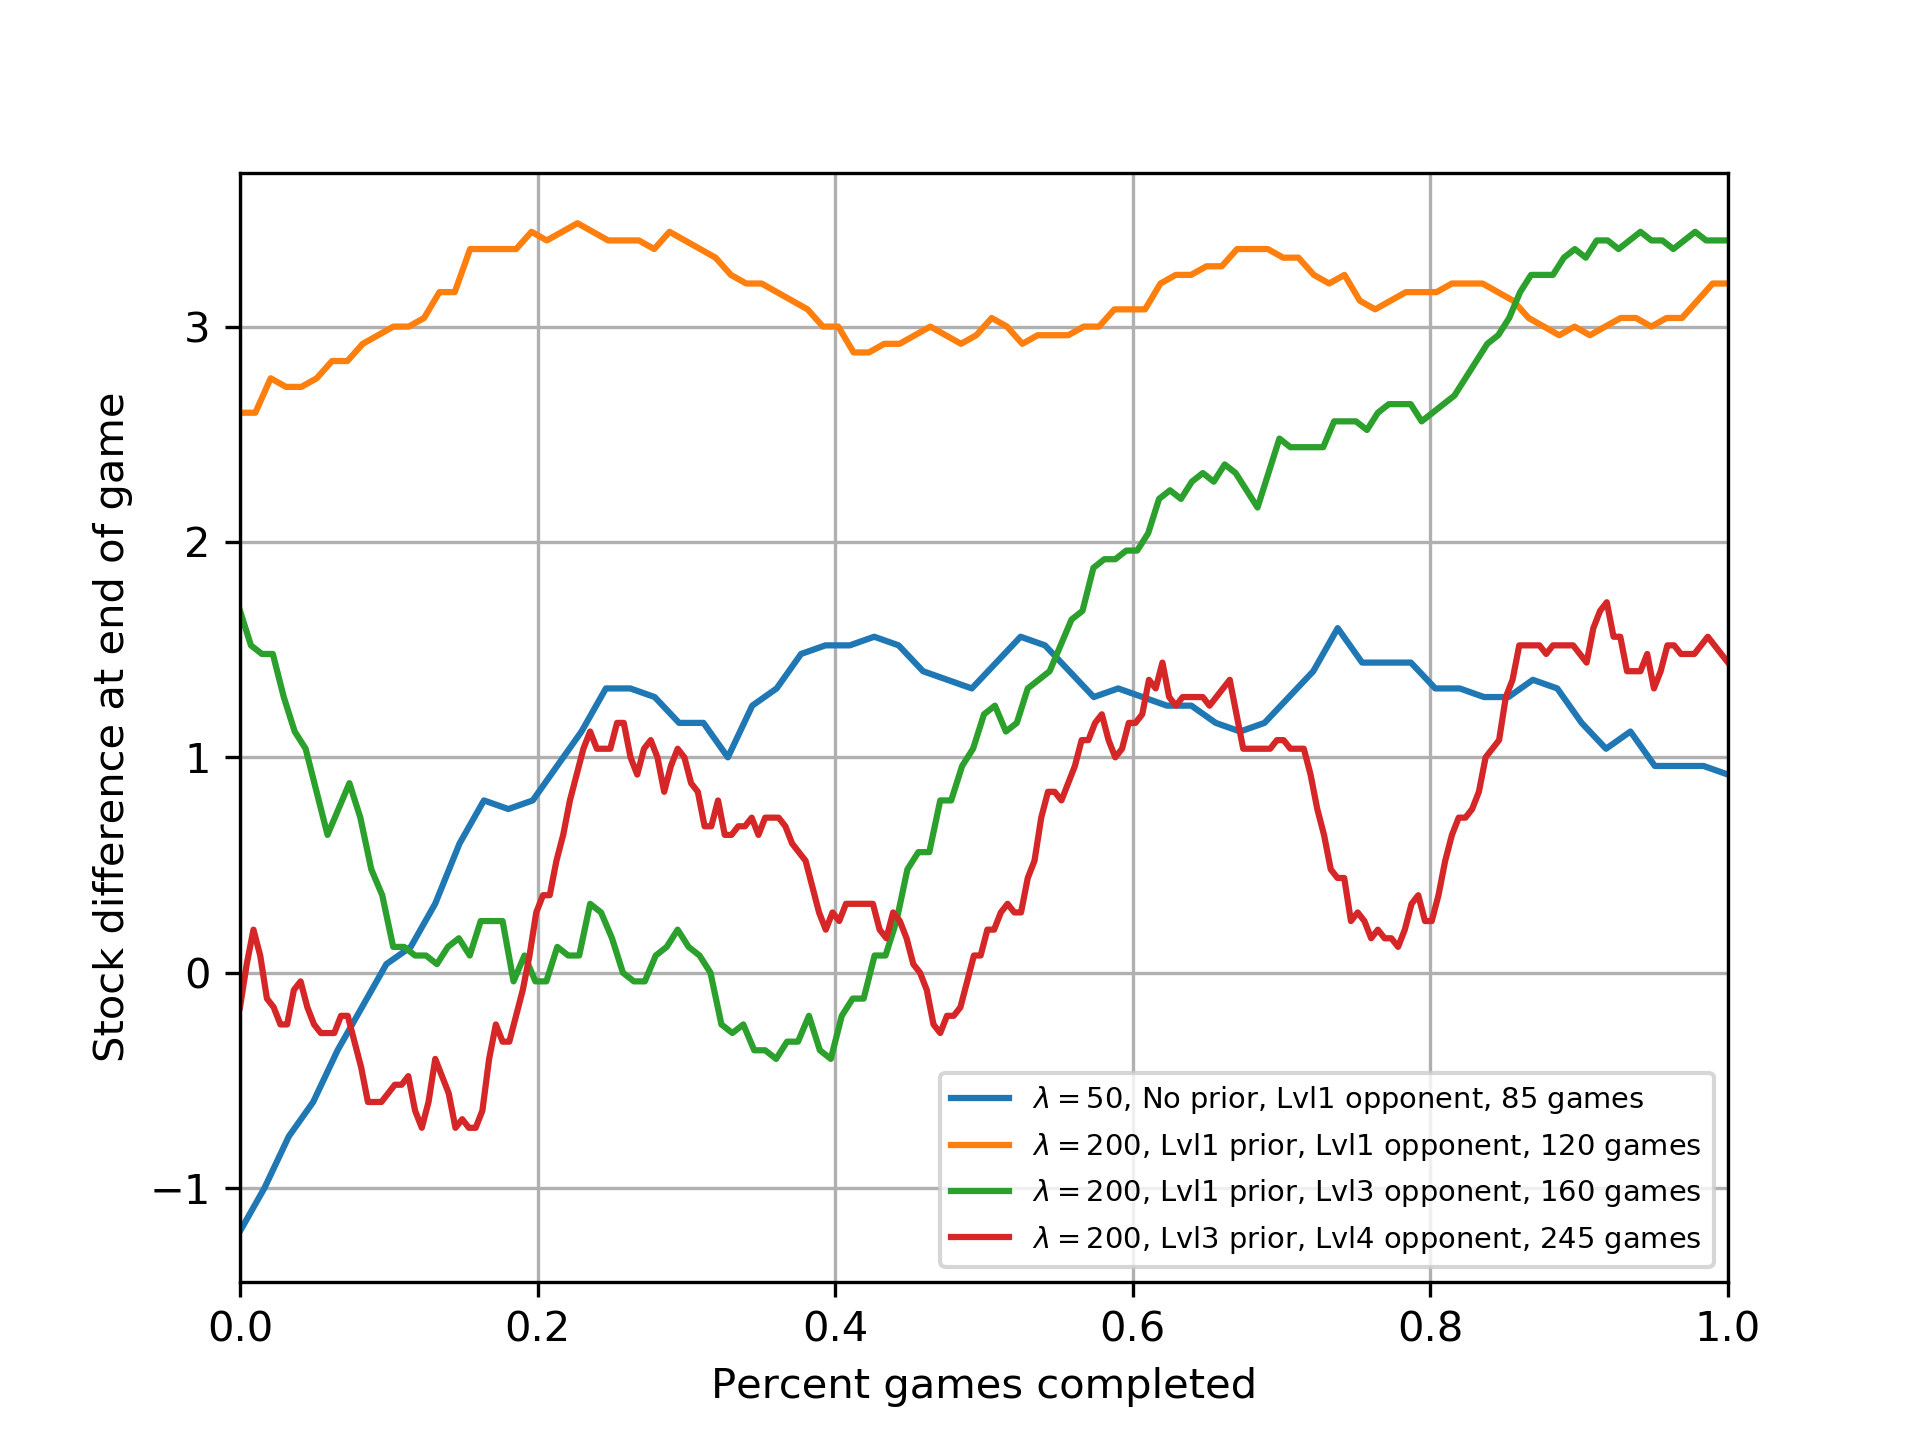
\includegraphics[width=120mm]{stocks.png}
	\caption{25 game moving average of stock differential at end of game (higher is better).\label{stocks}}
\end{figure}

\begin{figure}[!htb]
\centering
	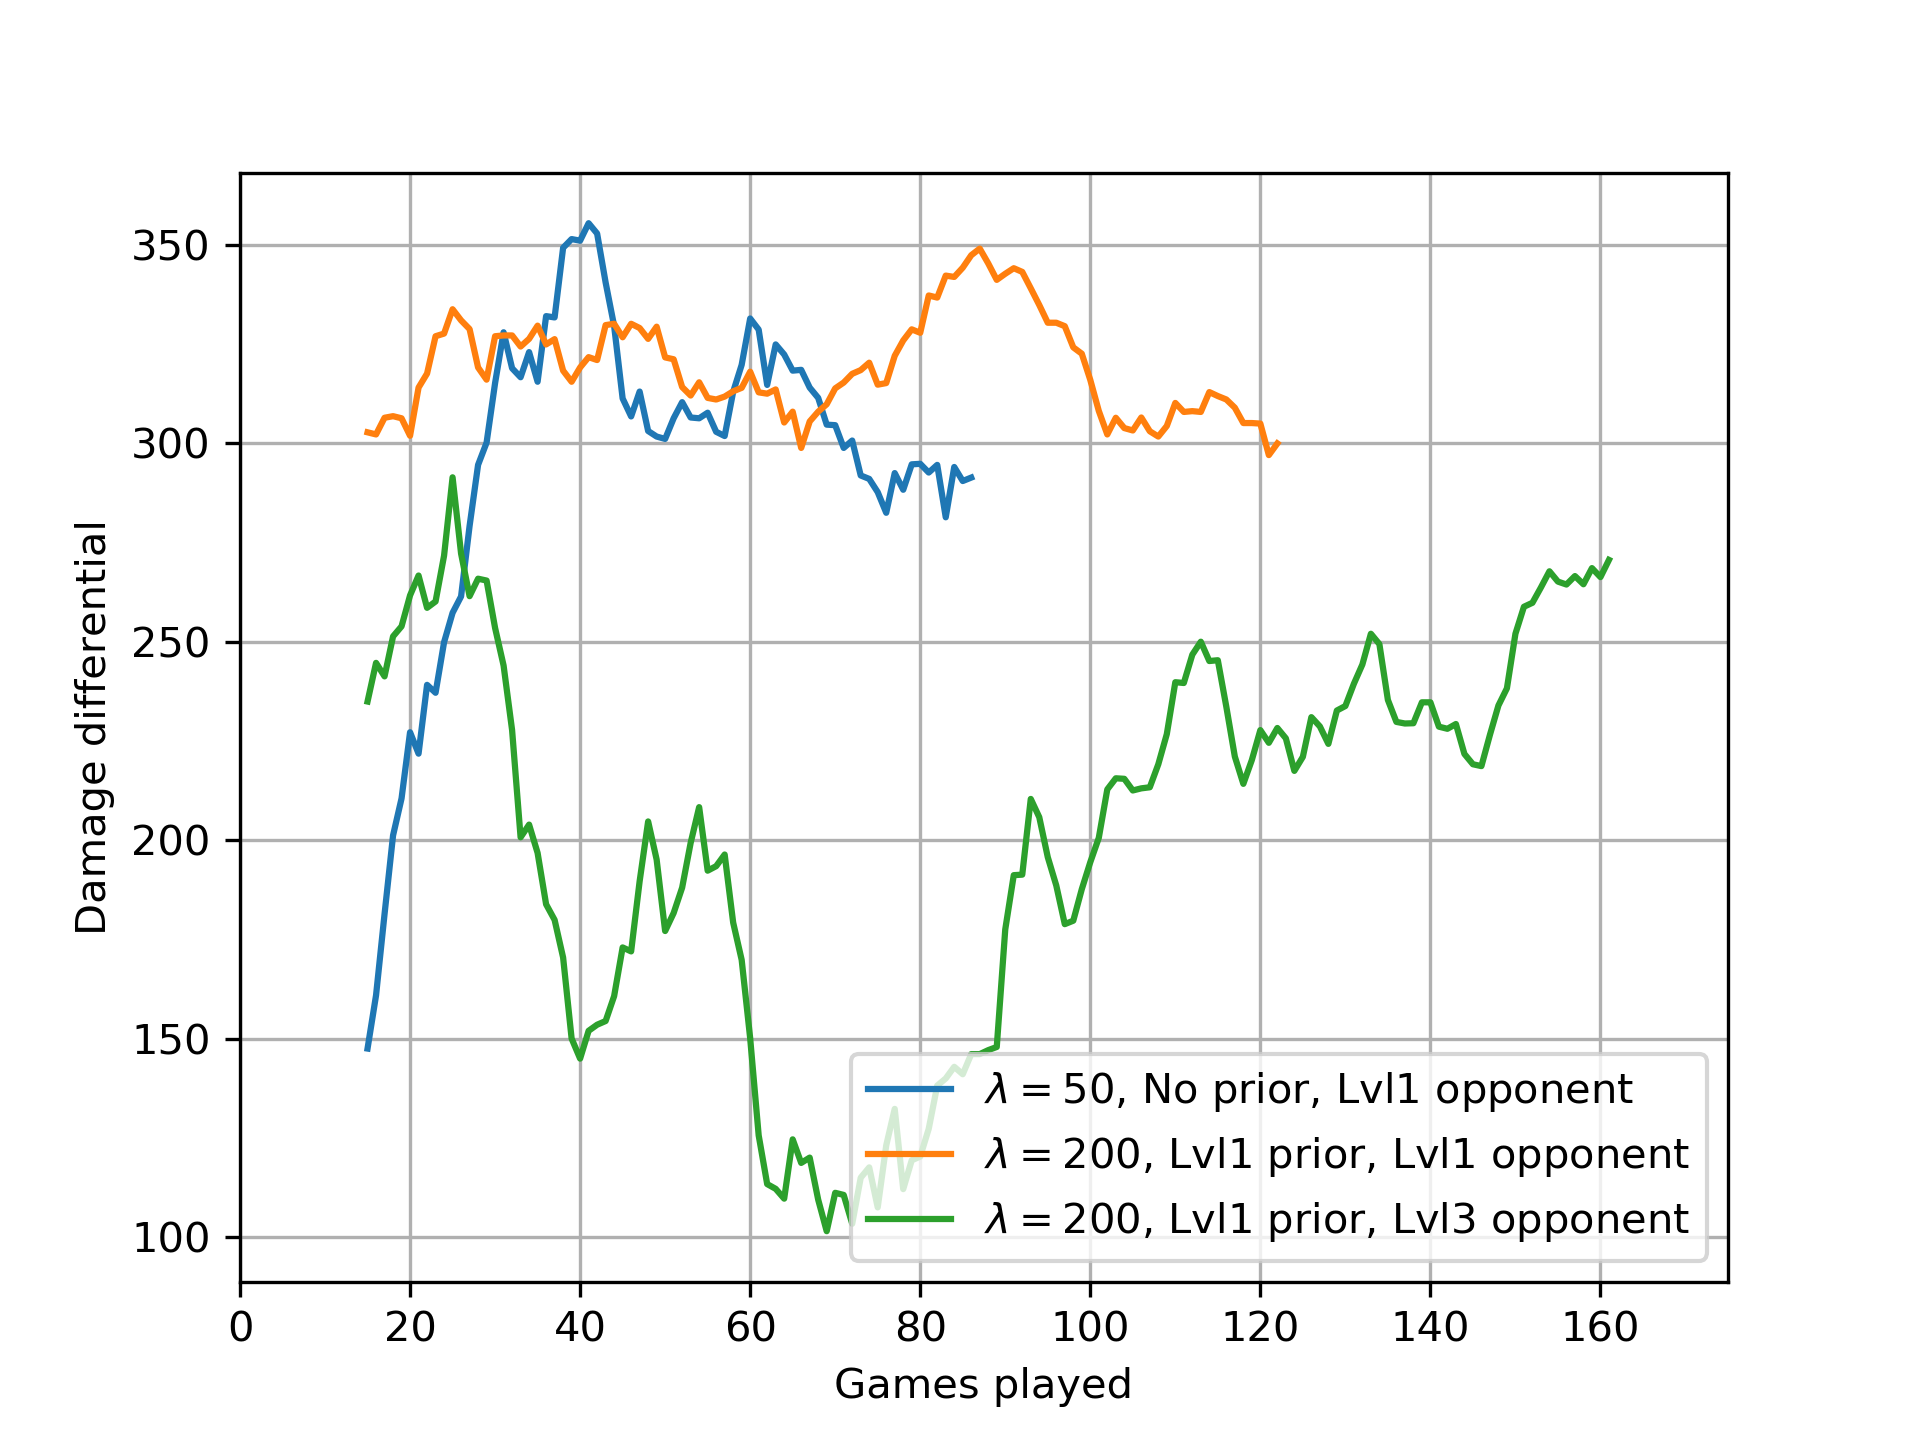
\includegraphics[width=120mm]{damage.png}
	\caption{25 game moving average of difference in total damage dealt in each game (higher is better). \label{damage}}
\end{figure}


%
% Acknowledgments
%
\section*{Acknowledgments}

We would like to acknowledge libmelee for providing an open source solution to obtaining information about the game while it is being played. We would also like to thank Professor Mykel Kochenderfer and the entire AA228 course staff for providing a fantastic learning experience. 

% add bibliography
% DONT DO BILBIO STYLE

\bibliography{biblio}

\end{document}
